\chapter{Public Financial Management}

\section*{Number of countries supported by DFID to manage their public finances (including natural resources and extractives) more transparently.}
% make sure numbers and header don't appear
\thispagestyle{empty}

\section{Results}

In 2019/120 DFID supported \textbf{39 countries} to manage their public finances (including natural resources and extractives) more transparently. %
This compares with 40 countries in 2018/19 and 39 countries in 2017/18. %

From 2015 to 2020 DFID continuously supported 26 countries to manage their public finances (including natural resources and extractives) more transparently.
%

\begin{figure}[htbp]
  \centering
  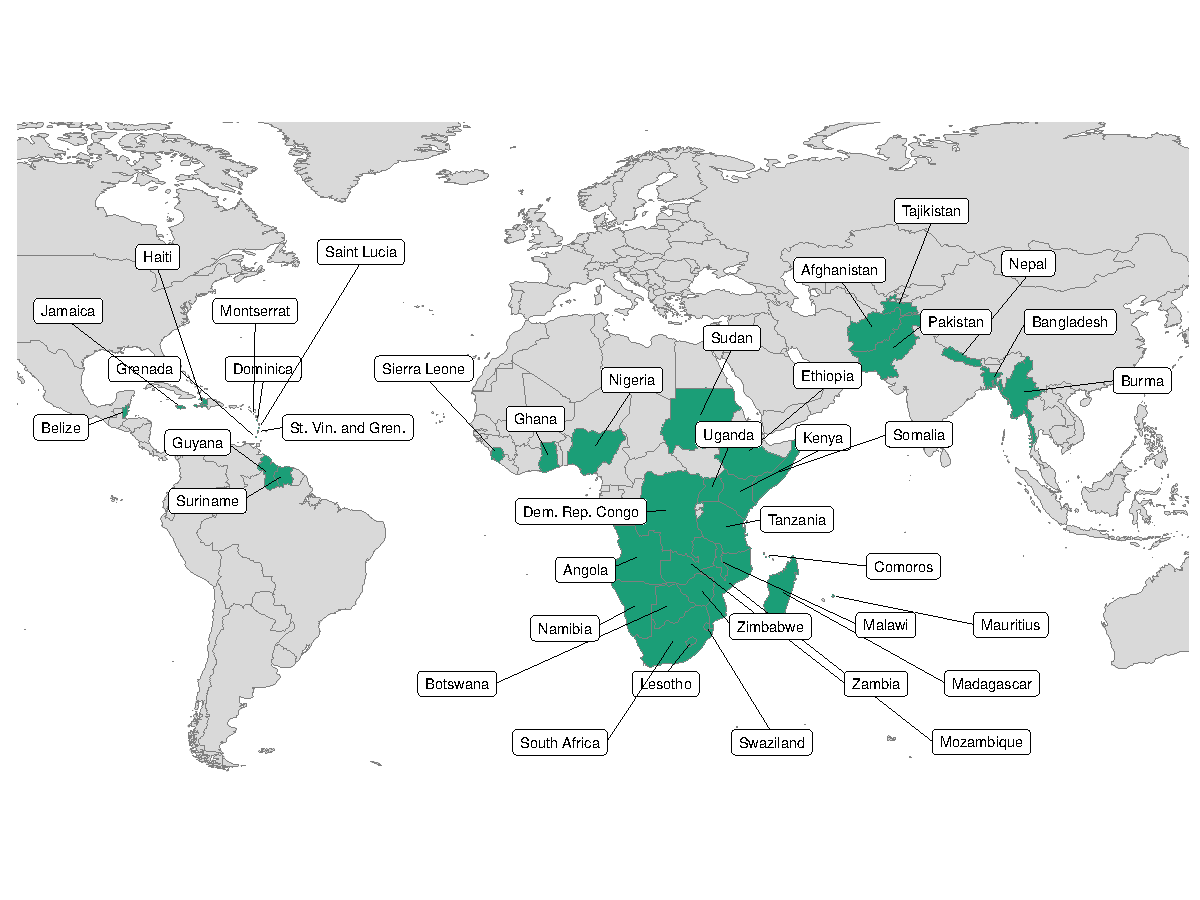
\includegraphics[width=0.95\textwidth]{../figs/pfm_plot} \hfill
  \caption{Countries supported in 2019/20 to manage their public finances more transparently.}
  \label{fig:pfm_plot}
\end{figure}


\section{Context}

Developing countries need to raise and utilise their own revenues to finance public services, and enable sustainable and inclusive growth and poverty reduction. %
Lack of transparency over Government budgeting makes it difficult to track spending, detect
misuse of public funds and hold decision makers to account. %

DFID support to improve fiscal transparency and accountability in developing countries is vital for a sustainable exit from aid, develops strong defence against corruption, and helps build capable and legitimate states, which are core to DFID's approach. %
This work also contributes towards delivery of the Sustainable Development Goals,
particularly Goal 16 (building `more effective and transparent institutions'). %

\newpage

